\documentclass[11pt]{beamer} %Add 'handout' in the options for printing

\usepackage{beamercolorthemewolverine}
\usetheme{AnnArbor}

\usepackage[english]{babel}
\usepackage{amsmath,amssymb}
\usepackage{mathtools}
\usepackage{commath}
\usepackage{amssymb,amscd,amsfonts,amsbsy}
\usepackage{enumerate}
\usepackage{epsfig}
\usepackage{pgfpages}
\usepackage{graphics}
\usepackage{graphicx}
\usepackage{multicol}
\usepackage{layouts}
\usepackage[center]{caption}
\usepackage{natbib}
%\usepackage{movie15}
\usepackage{etex}
\usepackage[export]{adjustbox}
\usepackage{embedfile}
\usepackage{caption}
\usepackage{soul,xcolor}
\usepackage{import}
\usepackage{relsize}
\usepackage{tikz}
\usepackage[makeroom]{cancel}
\usepackage{multimedia}
\usepackage{subcaption}
\usepackage{comment}
%\usepackage{media9}



%Setup note page
\setbeamertemplate{note page}[plain]
%\setbeameroption{show notes on second screen=right}
%\setbeameroption{show notes on second screen=left}

\setbeamertemplate{navigation symbols}{}%remove navigation symbols

\setbeamertemplate{footline}[frame number]{}%gets rid of bottom navigation bars


\graphicspath{ {../figs/lung_figs/} }


% Figures within a column...
\makeatletter
\newenvironment{tablehere}
{\def\@captype{table}}
{}
\newenvironment{figurehere}
{\def\@captype{figure}}
{}
\makeatother

\newcommand{\beginbackup}{
   \newcounter{framenumbervorappendix}
   \setcounter{framenumbervorappendix}{\value{framenumber}}
}
\newcommand{\backupend}{
   \addtocounter{framenumbervorappendix}{-\value{framenumber}}
   \addtocounter{framenumber}{\value{framenumbervorappendix}} 
}

%---------------------------------------------------------------------------
%\setbeamercolor{mycolor}{fg=White,bg=White}
\setbeamercolor{alerted text}{fg=red} 
\setbeamertemplate{frametitle}
{
  \vskip-5pt 
  \leavevmode
  \begin{center}
    \vspace*{-0.5cm}
  \hbox{%
  \begin{beamercolorbox}[wd=0.85\paperwidth,ht=0.35cm,dp=1.35ex]{White}%
    \raggedright
    \vspace*{-.25cm}
    {\normalsize \insertframetitle} %\small{\insertframetitle}
  \end{beamercolorbox}
  % \hspace*{1em}{\normalsize \insertframetitle} %\small{\insertframetitle}
  }%
  \end{center}
  \vspace*{-0.75cm}
}
\def\newblock{\hskip .11em plus .33em minus .07em}

\setbeamertemplate{headline}{}

\setbeamercovered{dynamic}


\newcommand{\RR}{{\mathbb{R}}}
\newcommand{\NN}{{\mathbb{N}}}
\newcommand{\ZZ}{{\mathbb{Z}}}
\newcommand{\CC}{{\mathbb{C}}}
\newcommand{\eps}{\varepsilon}
\newcommand{\bp}{\noindent {\it Proof}.\,\,\,}
\newcommand{\ep}{\hfill$\Box$ \vskip 0.08in}
\newcommand{\dint}{\int\!\!\!\int}
\newcommand{\vs}{\vskip 0.5cm}
\newcommand{\po}{{\partial\Omega}}
\newcommand{\meanint}{{\int{\mkern-19mu}-}}
\def\ring{\mathaccent"0017 }

\definecolor{AliceBlue}{RGB}{240,248,255}


%\definecolor{lightblue}{rgb}{1,0,0}
%\sethlcolor{lightblue}
\renewcommand<>{\hl}[1]{\only#2{\beameroriginal{\hl}}{#1}}

% http://tex.stackexchange.com/questions/41683/why-is-it-that-coloring-in-soul-in-beamer-is-not-visible
\makeatletter
\newcommand\SoulColor{%
  \let\set@color\beamerorig@set@color
  \let\reset@color\beamerorig@reset@color}
\makeatother
\SoulColor



%\usepackage{media9}%
%\newcommand{\includemovies}[3]{%
%\includemedia[%
%width=#1,height=#2,%
%activate=pagevisible,%
%deactivate=pageclose,%
%addresource=#3,%
%flashvars={%
%src=#3 % same path as in addresource!
%&autoPlay=true % default: false; if =true, automatically starts playback after activation (see option ‘activation)’
%&loop=true % if loop=true, media is played in a loop
%&controlBarAutoHideTimeout=0 %  time span before auto-hide
%}%
%]{}{StrobeMediaPlayback.swf}%
%}



%%% Local Variables:
%%% mode: latex
%%% TeX-master: "../main"
%%% End:

\embedfile{\jobname}
\embedfile{include/preamble.tex}
%

% My commands
\newcommand{\orderof}[1]{\ensuremath{\mathcal{O}\left(#1\right)}}

\begin{document}
%% Some customizations, based on https://tex.stackexchange.com/questions/22346/how-to-customize-titlepage-in-beamer

% \defbeamertemplate*{title page}{customized}[1][]
% {
% %  \usebeamerfont{title}\inserttitle\par
% %  \usebeamerfont{subtitle}\usebeamercolor[fg]{subtitle}\insertsubtitle\par
% %  \bigskip
%  % \usebeamerfont{author}\insertauthor\par
% %  \usebeamerfont{institute}\insertinstitute\par
% %  \usebeamerfont{date}\insertdate\par
%   \usebeamercolor[fg]{titlegraphic}\inserttitlegraphic
% }


%%
\title[]{Applications of Computation in Acoustics:\\Ultrasound Bioeffects \&\\ Underwater Transmission Loss Uncertainty}
\author[] {}

\institute[]{}
\date[date]{}


\begin{frame} %\vspace{1cm}
  \vspace*{1cm}
  %\titlepage \vspace{-2.50cm}

  {
    %\definecolor{darkpowderblue}{rgb}{0.0, 0.2, 0.6} %% UNCOMMENT IF NOT IN PREAMPLE
    \setbeamercolor{title}{fg=white, bg=darkpowderblue}
  \begin{beamercolorbox}[sep=8pt,center,wd=\paperwidth,ht=0.3\textheight,dp=0.045\textheight]{title}
    \usebeamerfont{title}\inserttitle\par%
  \end{beamercolorbox}
  }
  \centering
  \begin{columns}
    \column{.25\textwidth}
    
    % \begin{figure}\vspace*{1.3cm} \centering 
\includegraphics[width=.70\columnwidth]{include/figs/MichiganSeal} \end{figure}
    \column{.5\textwidth}
    \begin{center}
      % 
      \normalsize{A \emph{dissertation defense} by:\\Brandon Patterson} \vspace{16pt} \\ 
      % 
      \footnotesize{Scientific Computing and Flow Physics Lab} \vspace{4pt}\\
      \footnotesize{University of Michigan, Ann Arbor} \vspace{4pt}\\
      \scriptsize{Department of Mechanical Engineering} \vspace{4pt}\\
      % \scriptsize{$^2$Department of Radiology} \vspace{4pt}
    \end{center}
    \column{.25\textwidth}
    \vspace*{.15cm}
    % \begin{figure} \vspace*{1.3cm} \centering 
\includegraphics[width=.70\columnwidth]{include/figs/MElogo} \end{figure}
  \end{columns}
  \vspace{.25cm}
  \begin{center}
    % 
    % 
    %%%%%%%%%%%%%%%%%%% Put Date Here   %%%%%%%%%%%%%%%%%%%%%%%%%%%%
    % \footnotesize {\today} \vspace{-.1cm}
    \footnotesize {October 31, 2017} \vspace{-.1cm}
    % 
    % 
  \end{center}



  % 
  % 
  %%%%%%%%%%%%%%%%%%% FUNDING SOURCE OR CONFERENCE IMAGES BELOW ( L | C | R )   %%%%%%%%%%%%%%%%%%%%
  \begin{minipage}{\textwidth}
    \hspace*{.5cm}
    \begin{minipage}{.3\textwidth}
      \begin{center} 
        \begin{figure}
          \centering
          % \includegraphics[width=.4\textwidth]{include/figs/NIH_logo}
          %	\label{fig:NIH_logo_blue}
        \end{figure}
      \end{center}
    \end{minipage}
    \begin{minipage}{.3\textwidth}
      \begin{center} 
        \begin{figure}
          \centering
          % \includegraphics[width=.8\textwidth]{include/figs/nsfgrfp}
          \label{fig:NSF_logo_blue}
        \end{figure}
      \end{center}
    \end{minipage}
    \begin{minipage}{.3\textwidth}
      \begin{center} 
        
      \end{center}
    \end{minipage}
  \end{minipage}
\end{frame}
%%% Local Variables:
%%% mode: latex
%%% TeX-master: "../main"
%%% End:




%%%%%%%%%%%%%%%%%%%%%%%%%%%%%%%% Slides %%%%%%%%%%%%%%%%%%%%%%%%%%%%%%
\begin{frame}
  \centering
  \begin{center}
    \hl{Sponsors slide}
  \end{center}
\end{frame}
%%
%%

\begin{frame} \frametitle{My work has focused on two very different problem areas within acoustics.}
  \begin{minipage}{0.48\textwidth}
    \begin{figure}
      Acoustic uncertainty in the ocean \vspace*{4pt}\\
      \centering
      \includegraphics[width=\textwidth]{./figs/bathmap}
    \end{figure}
  \end{minipage}
  \hfill
  \begin{minipage}{0.48\textwidth}
    \begin{figure}
      \centering
      Ultrasound bioeffects \vspace*{4pt}\\
      \includegraphics[width=\textwidth]{./figs/ultrasound_example}
    \end{figure}
  \end{minipage}
\end{frame}
%%
%%
\begin{frame} \frametitle{\textit{Past work}: Efficient estimation of the probability density function of transmission loss in uncertain ocean environments}
{\small
\vspace*{0.25cm}
Transmission Loss, $TL=20log_{10}\left(\frac{p_{source}}{p_{receiver}}\right)$, is useful for naval applications.
\vspace*{0.25cm}
\begin{figure}
  \centering
  \includegraphics[width=0.6\textwidth]{./figs/ocean_0}
\end{figure}
TL uncertainty is important for those making decisions based on TL,
but traditional methods are slow and expensive.  \hl{Add features to
  ocean} }
\end{frame}
%%
%%
\begin{frame} \frametitle{\textit{Past work}: We developed a computationally efficient way of computing TL in uncertain environments}
  \begin{figure}\hfill
    \includegraphics[height=0.3\textheight]{./figs/as_ocean_schematic}\hfill
    \visible<2->{\includegraphics[height=0.32\textheight]{./figs/as_field}}\hfill
    \visible<3->{\includegraphics[height=0.32\textheight]{./figs/as_subfield}}\hfill
  \end{figure}
  \vspace{-0.7cm}
  \begin{figure}
    \visible<4->{\includegraphics[height=0.3\textheight]{./figs/as_hist}}\hfill
    \visible<5->{\includegraphics[height=0.3\textheight]{./figs/as_mc_tlpdf}}\hfill
    \visible<6->{\includegraphics[height=0.32\textheight]{./figs/tl_success_field_labeled}}\hfill
  \end{figure}
  \vspace{-0.5cm}
  {\footnotesize
    \visible<7->{
    \begin{itemize}
    \item Engineering level accurate $\left(L_1\text{-error}<0.5\right)$ in 93\% of test cases in bottom reflecting environments. \vspace*{-4pt}
    \item $\approx \orderof{10^{-6}}$ the cost of 1000-sample Monte Carlo Methods.
    \end{itemize}
  }
  }
\end{frame}
%%
%%
\begin{frame} \frametitle{Background on medical ultrasound}
  \begin{itemize}
    \item High frequency sound waves travel into the body and scatter at material interfaces.
    \item Much of the acoustic energy is dissipated as heat.
  \end{itemize}
\end{frame}
%%
%%
\begin{frame} \frametitle{Background on diagnostic ultrasound}
  \begin{itemize}
    \item Diagnostic Ultrasound (DUS) is ubiquitous and generally very safe
    \item Lung Hemorrhage (LH) is the only known bioeffect of non-contrast diagnostic ultrasound
  \end{itemize}
\end{frame}
%%
%%
\begin{frame} \frametitle{Background on ultrasound-bioeffects}
  \begin{itemize}
    \item Diagnostic Ultrasound (DUS) is ubiquitous and generally very safe
    \item Lung Hemorrhage (LH) is the only known bioeffect of non-contrast diagnostic ultrasound
  \end{itemize}
\end{frame}
%%
%%
\begin{frame} \frametitle{\textit{Past work}: Theoretical microbubble dynamics in a viscoelastic medium at capillary breaching thresholds}
\vspace*{\fill}
  \begin{minipage}{\textwidth}
    \begin{minipage}{0.3\textwidth}
      \begin{figure}
        \centering
        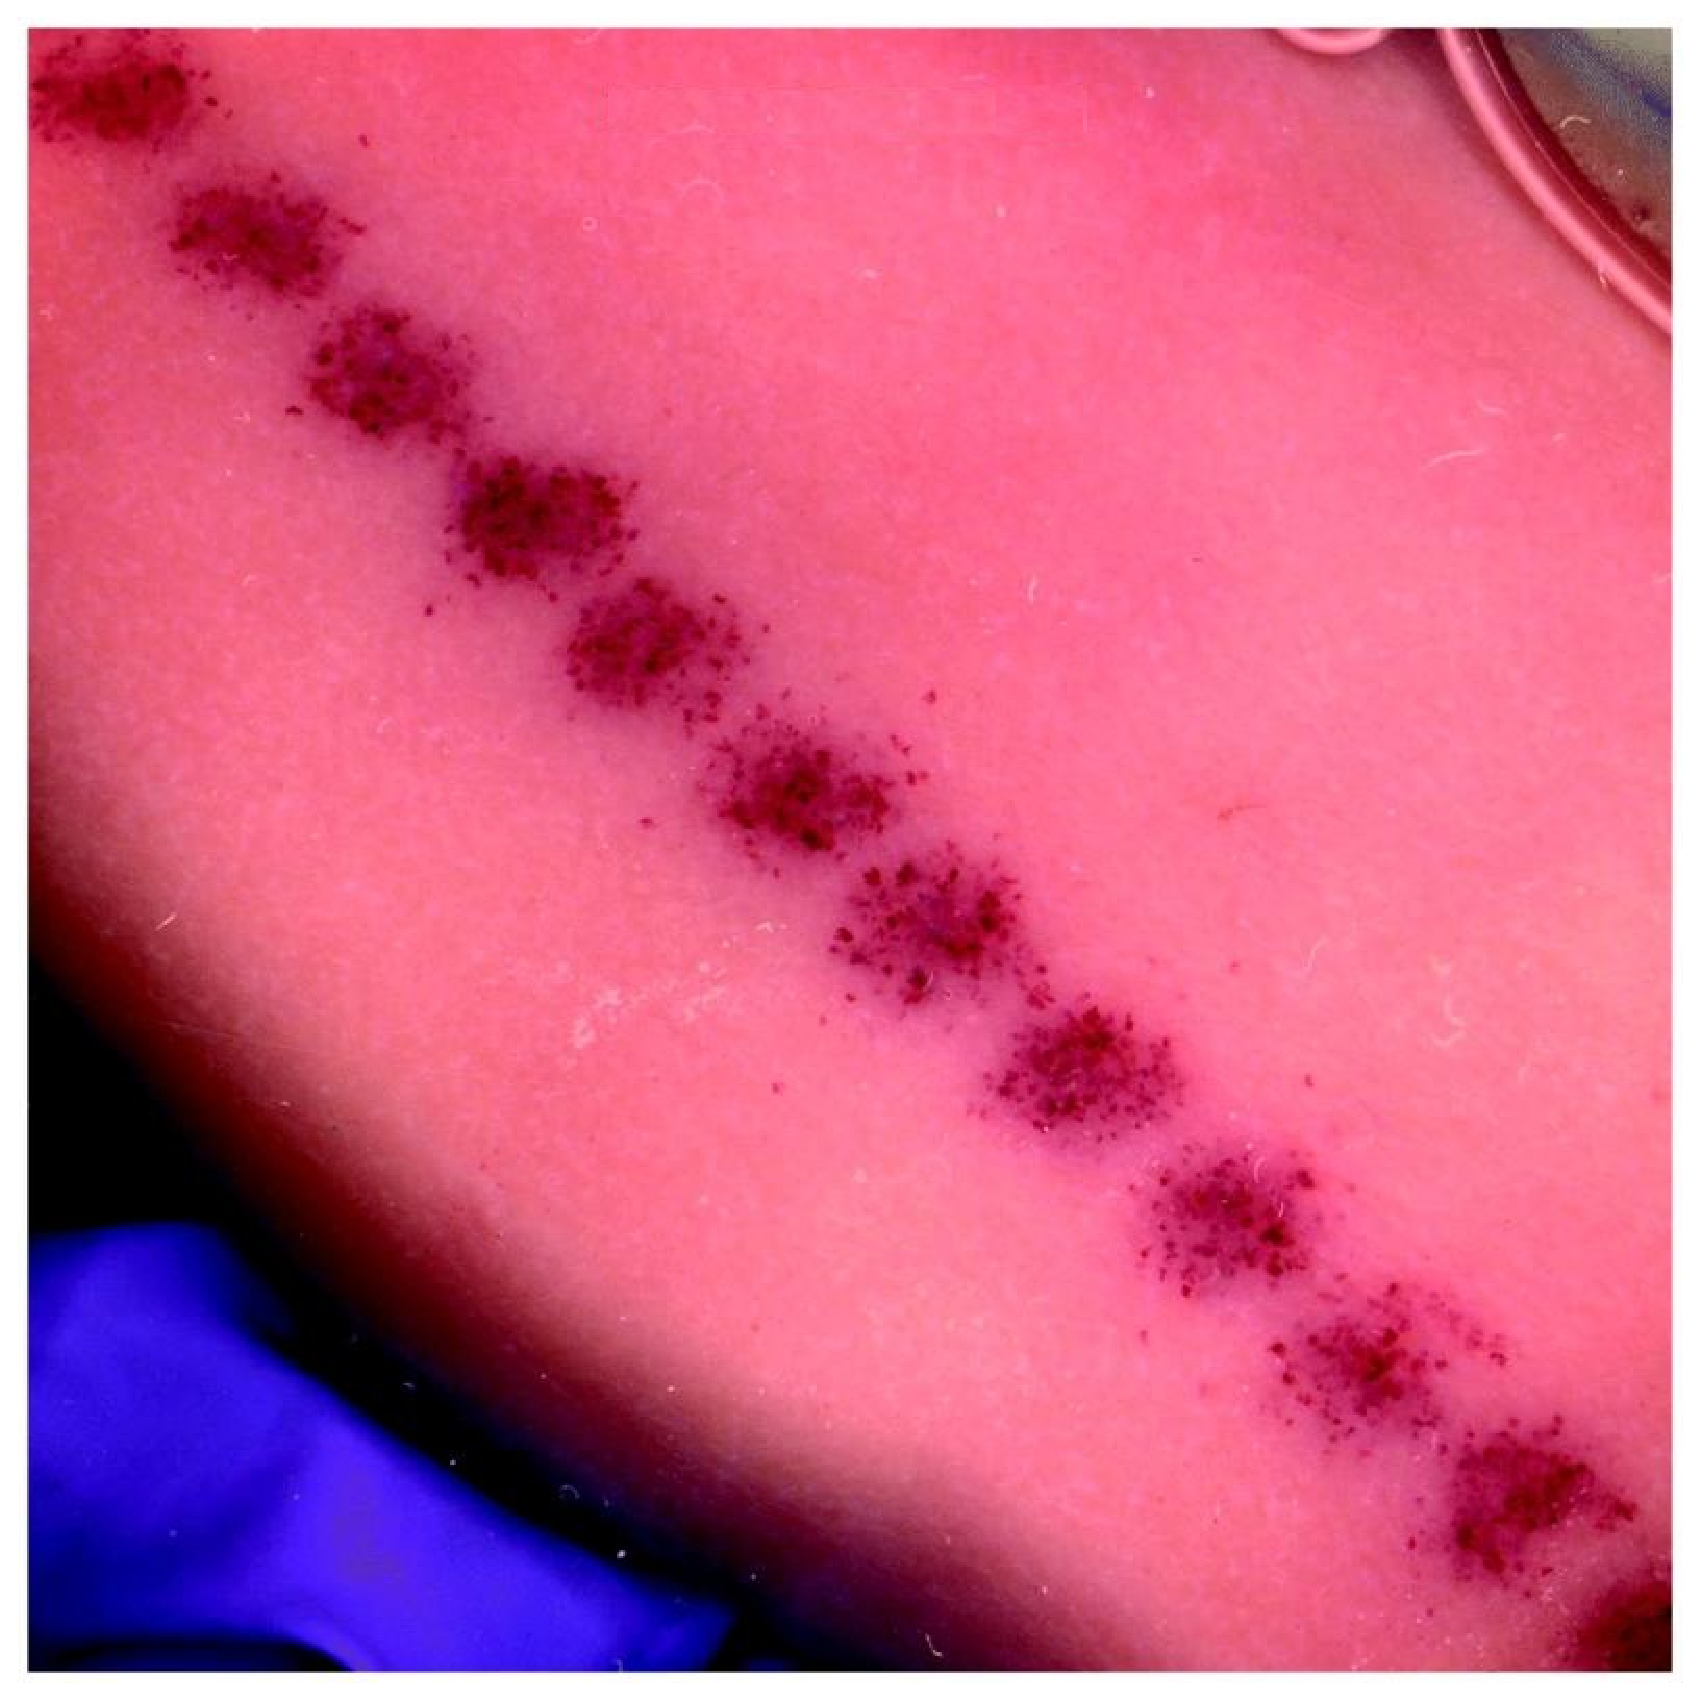
\includegraphics[width=0.8\textwidth]{./figs/Kidney_Bleed}
      \end{figure}
    \end{minipage}
    \begin{minipage}{0.68\linewidth}
    {\tiny
      \scalebox{0.9}{$
        \left(1-\frac{\dot{R}}{C}\right) R \ddot{R} + \frac{3}{2}\left(1-\frac{\dot{R}}{3 C}\right) \dot{R}^2 = \left(1+\frac{\dot{R}}{C}\right) \left[p_B- 1 -p_a -
          \frac{R}{C}\frac{dp_a}{dt}\right] +\frac{R}{C} \dot{p}_B,$\\}%
      \vspace*{2pt}
      \scalebox{0.9}{$p_B = \left(1+\frac{2}{We}\right)\frac{1}{R^{3\gamma}}-\frac{2}{WeR} + \tau_R,$\\}

      \vspace*{0.5cm}
      \begin{tabular}{l l c l}
        Parameter & Dimensional value & & Dimensionless number \\ \hline
        Viscosity & $\mu=0.015$ (Pa s) & $\mapsto$ & $Re=\rho u R_o / \mu = 2/3$ \\
        Elasticity & $G=10^5$ (Pa) & $\mapsto$ & $Ca= \rho u^2 / G = 1.0$ 	\\
        Surface tension & $S=0.056$ (N/m) & $\mapsto$ & $We=\rho u^2 R_o / S$ = 2 \\
        Sound speed & $c=1570$ (m/s) & $\mapsto$ & $C = c/u=157$ \\  
        % Relaxation time & $\lambda = 0.5$ ($\mu$ s) & $\mapsto$ &	$De=\lambda u / R_o =0$ \\
      \end{tabular} 
    }
    \end{minipage}
  \end{minipage}

  \vfill

  \begin{minipage}{\textwidth}
    \includegraphics[width=0.6\textwidth]{../figs/bubble_figs/rt_nonlinear}\hfill
    \includegraphics[width=0.33\textwidth]{../figs/bubble_figs/rstarmax_f}  
  \end{minipage}
\end{frame}
%%
%%
\begin{frame}
  \centering
  \begin{center}
    {\LARGE Part II: Current Project}\\
    
    Diagnostic ultrasound-induced lung hemorrhage and acoustic wave
    interactions with liquid-gas interfaces
  \end{center}
\end{frame}
%%
%%
\begin{frame} \frametitle{Background on wave-interface interaction}

\end{frame}
%%
%%
\begin{frame} \frametitle{Diagnostic ultrasound-induced lung hemorrhage is not a new problem}
{\small
  \begin{itemize}
  \item Lung Hemorrhage (LH) is the only known bioeffect of non-contrast Diagnostic UltraSound (DUS).
  \item Has been shown to occur in mice, rats, pigs, rabbits, monkeys \citep{Child1990,OBrien1997a,OBrien2001,Tarantal1994a}.
  \end{itemize}
}
\vspace{-0.5cm}
  \begin{figure}
    \centering
    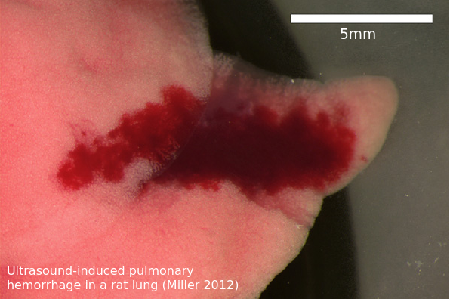
\includegraphics[width=0.5\textwidth]{LungBleed2} \nocite{Miller2012}
  \end{figure}
\vspace{-0.35cm}
The underlying physical damage mechanism is still unknown.
%
\end{frame}
%%
%%
\begin{frame} \frametitle{Shock-driven fluid-fluid interfaces have been studied extensively}
  \begin{itemize}
  \item 
  \end{itemize}
\end{frame}
%%
%%
\begin{frame}
We aim to study acoustic wave interactions with perturbed liquid-gas interfaces
\end{frame}
%%
%%
\begin{frame} \frametitle{Methods: Problem setup}
  \begin{figure}
    \centering
    \def\svgwidth{0.48\textwidth}
    {\footnotesize
    \import{../figs/lung_figs/}{usbe_lung_schematic2.pdf_tex} \hfill%
  }
    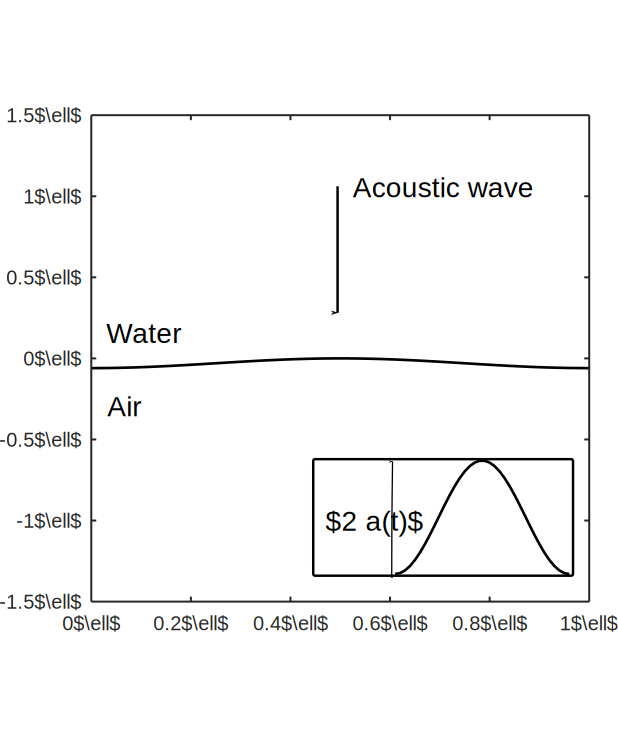
\includegraphics[width=0.48\textwidth]{../figs/lung_figs/usbe_model_schematic} \hfill
  \end{figure}
\end{frame}
%%
%%
\begin{frame} \frametitle{Methods: The acoustic waves}
  \begin{figure}
    \centering
      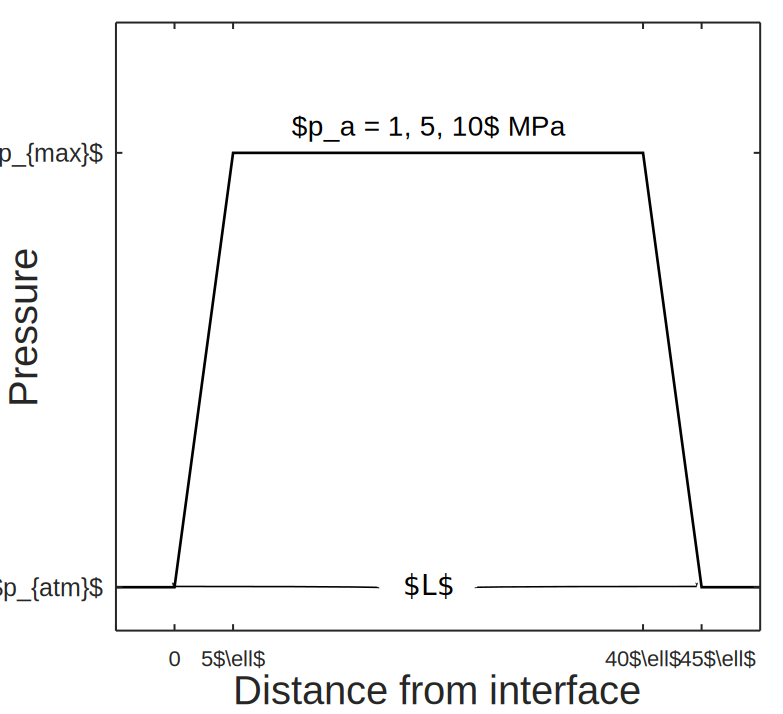
\includegraphics[width=0.47\textwidth]{../figs/lung_figs/p0_vs_y}%
      \includegraphics[width=0.47\textwidth]{../figs/lung_figs/p0_vs_t_us}%
  \end{figure}
\end{frame}
%%
%%
\begin{frame} \frametitle{Methods: Governing Equations}
Euler equations of fluid motion
  \begin{align*}% 
    \frac{\partial \rho}{\partial t} + \frac{\partial \left(\rho u\right)}{\partial x} + \frac{\partial \left(\rho v\right)}{\partial y} = 0,\\
    \frac{\partial \rho u}{\partial t} + \frac{\partial}{\partial x}\left( \rho u^2+p\right)  + \frac{\partial}{\partial y}\left( \rho uv\right) = 0,\\
    \frac{\partial \rho v}{\partial t} + \frac{\partial}{\partial x}\left( \rho uv\right)  + \frac{\partial}{\partial y}\left( \rho v^2+p\right) = 0,\\
    \frac{\partial E}{\partial t} + \frac{\partial}{\partial x}\left[u\left(E+p\right)\right] + \frac{\partial}{\partial y}\left[v\left(E+p\right)\right] = 0,
  \end{align*}%

Stiffened equation of state
\begin{align*} \label{eq:stiffened_eos}%
  E=\frac{\rho\left(u^2+v^2\right)}{2} + \frac{p+\gamma B}{\gamma-1}.
\end{align*}
% Two additional advection equations are solved for $\gamma$ and $B$.
\end{frame}


%%
%%
\begin{frame} \frametitle{Methods: Computational techniques}
  \begin{figure}
    \centering
    
  \end{figure}
\end{frame}
%%
%%
\begin{frame} \frametitle{Results: Evolution of the interface}
  \begin{figure}
    \centering
    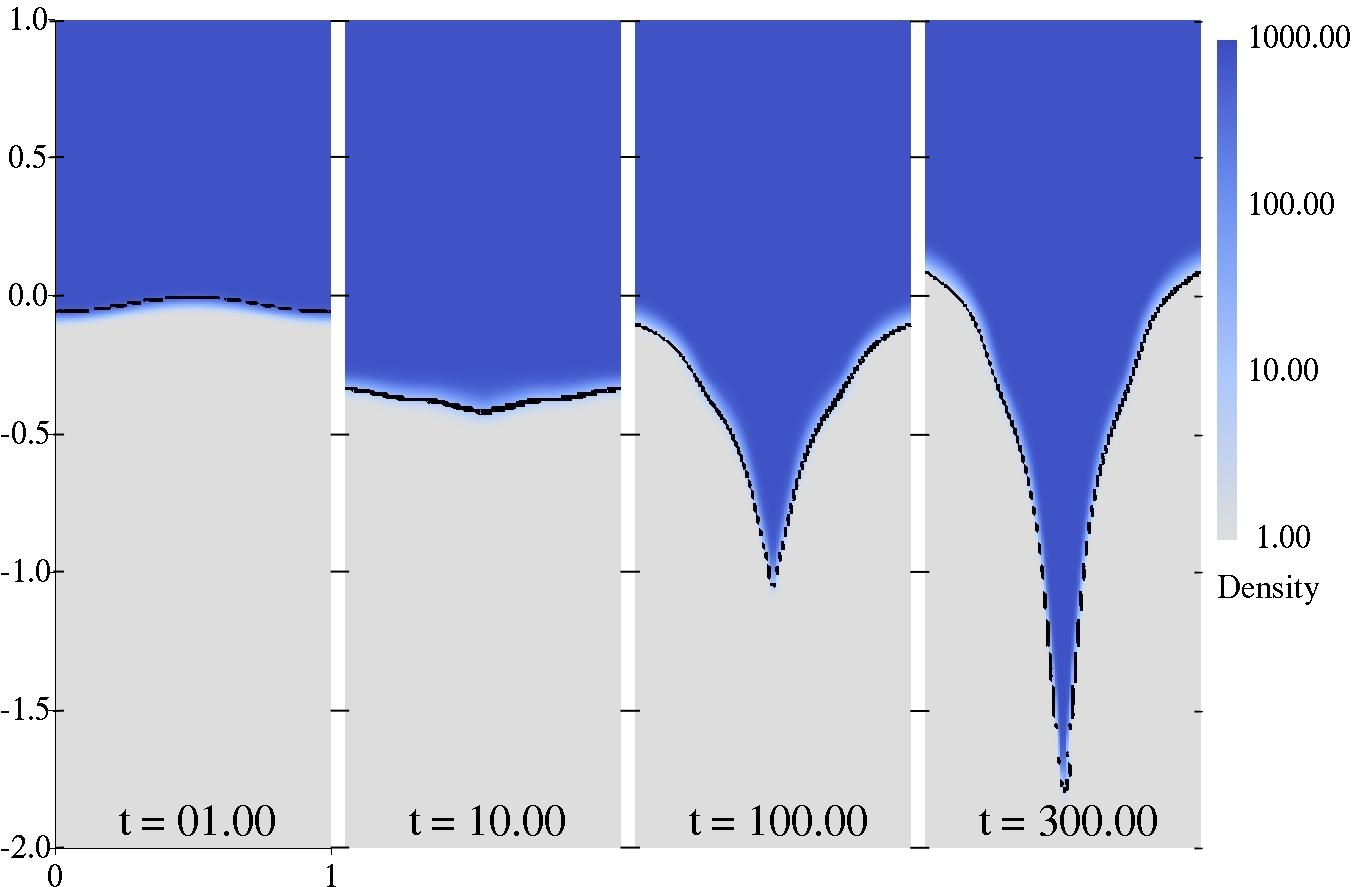
\includegraphics[width=0.9\textwidth]{../figs/lung_figs/snapshots_density_t1}
  \end{figure}
\end{frame}
%%
%%
\begin{frame} \frametitle{Results: Evolution of the interface}
  \begin{figure}
    \centering
    \includegraphics[width=0.48\textwidth]{../figs/lung_figs/trapz10_intf_schematic}
    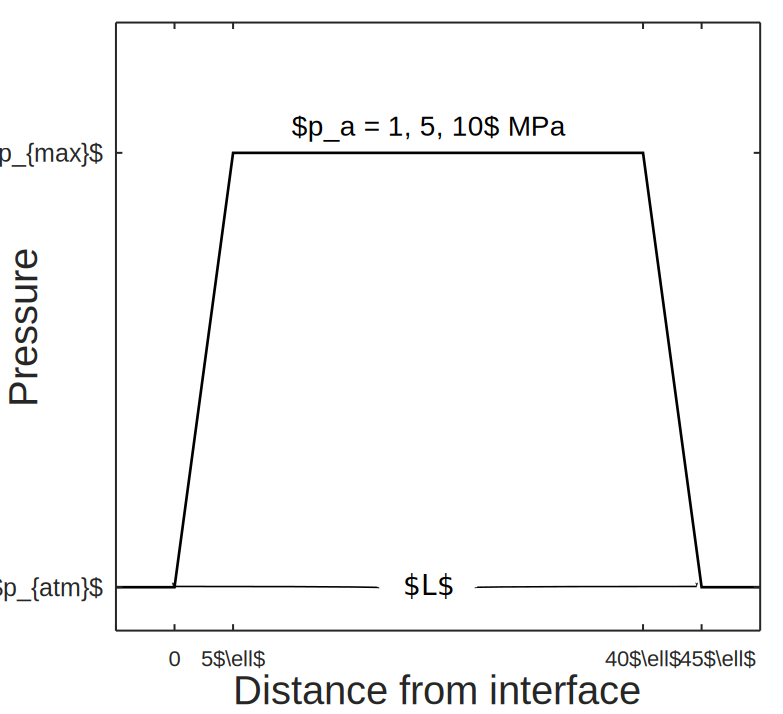
\includegraphics[width=0.47\textwidth]{../figs/lung_figs/p0_vs_y}%
  \end{figure}
\end{frame}
%%
%%
\begin{frame} \frametitle{Results: Late-time evolution of the interface}
  \begin{minipage}{0.5\textwidth}
    \begin{figure}
      \centering
      \includegraphics[width=\textwidth]{../figs/lung_figs/interface_multi-amp_loglog_roe_extra}
    \end{figure}
  \end{minipage}
  \hfill
  \begin{minipage}{0.48\textwidth}
    \begin{align*}
      a(t) \sim \sqrt{\Gamma t}.
    \end{align*}
  \end{minipage}
\end{frame}
%%
%%
\begin{frame} \frametitle{Results: Vorticity dynamics}
  \begin{figure}
    \centering
    \includegraphics[width=0.8\textwidth]{../figs/lung_figs/snapshots_vorticity_t1}
  \end{figure}
%
  \begin{itemize}
  \item Two questions: What kinds of vorticity, can we predict where it is generated
  \end{itemize}
\end{frame}
%%
%%
\begin{frame} \frametitle{Results: Evolution of the interface}
  \begin{figure}
    \centering
    \includegraphics[width=0.48\textwidth]{../figs/lung_figs/trapz10_circ_schematic}
    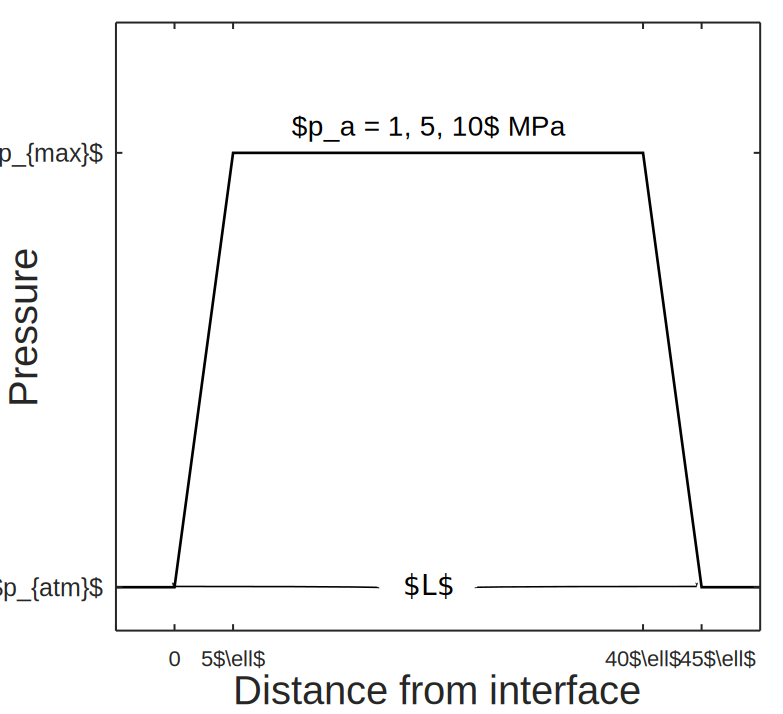
\includegraphics[width=0.47\textwidth]{../figs/lung_figs/p0_vs_y}%
  \end{figure}
\end{frame}
%%
%%
\begin{frame} \frametitle{Analysis of vorticity dynamics}%
  \begin{align*}
  \frac{\partial \vec{\omega}}{\partial t}+\left(\vec{u}\cdot\nabla\right)\vec{\omega} =% 
  - \vec{\omega}\left(\nabla\cdot\vec{u}\right) + \frac{\nabla\rho\times\nabla p}{\rho^2}.%
  \end{align*}
\end{frame}
%%
%%
\begin{frame} \frametitle{Results: Vorticity dynamics}
  \begin{itemize}
  \item Surface plot of vorticity during the compression wave interaction
  \item Plot of vorticity vs time (during wave interaction)
  \item Vorticity distribution plots
  \end{itemize}
\end{frame}
%%
%%
\begin{frame} \frametitle{Vorticity generation occurs primarily in gas-dominated fluid}
\vspace*{-.5cm}
{\scriptsize
    \begin{figure}
    \centering
    \hfill
    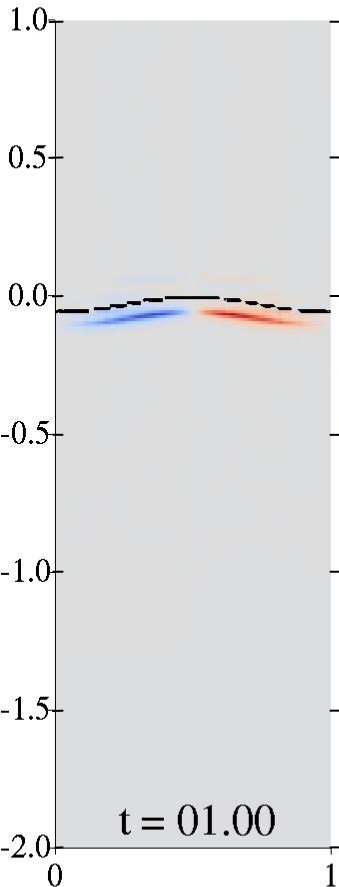
\includegraphics[width=.13\textwidth]{../figs/lung_figs/snapshots_vorticity_t1_only} \hfill
    \includegraphics[width=.38\textwidth]{./figs/vorticity_vs_y0} \hfill
    \includegraphics[width=.38\textwidth]{./figs/circ_y0_dist}
    \hfill
  \end{figure}
  %
  \vspace*{-.3cm}
  \begin{align*}%
    \frac{\norm{\frac{\nabla\rho\times\nabla p}{\rho^2}}_{air\quad}}{\norm{\frac{\nabla\rho\times\nabla p}{\rho^2}}_{water}}%
    =&\orderof{\abs{\boldsymbol{T}}\left(\frac{\abs{\rho^-}}{\abs{\rho^+}}\right)^2}%
    \approx 357
  \end{align*}
  \vspace*{-.25cm}
  % 
  \begin{itemize}
    \item 97\% of circulation appears in fluid with $y_0<0.5$
    \item Computed circulation ratio from air($y_0<0.1$) to water($y_0>0.9$) is $\approx 27$
  \end{itemize}
}
\end{frame}
%%
%%
\begin{frame} \frametitle{Interface response to a 10 MPa DUS pulse}
  \begin{figure}
    \centering
    \includegraphics[width=0.48\textwidth]{../figs/lung_figs/us_intf_schematic} \hfill
    \includegraphics[width=0.48\textwidth]{../figs/lung_figs/us_circ_schematic}
  \end{figure}
\end{frame}
%%
%%
\begin{frame} \frametitle{Conclusions thus far}
  \begin{itemize}
  \item Acoustically-generated baroclinic vorticity is likely capable
    of significantly deforming perturbed liquid gas interfaces.
  \item Baroclinic vorticity is predominantly deposited in gaseous fluids.
  \item Changes in the acoustic waveform that have little effect on
    the interface during the wave-interface interaction can
    substantially effect the interface over long periods of time, via
    vorticity.
  \end{itemize}
\end{frame}
%%
%%
\begin{frame}
  \centering
  \begin{center}
    \LARGE Part III: Future work
  \end{center}
\end{frame}
%%
%%
\begin{frame}\frametitle{I aim to increase the relevance to DUS}
  \begin{itemize}
  \item Calculate the engineering strain of the interface
  \item Calculate the stress at the interface
  \item Investigate the effects of alveolar side wall structures
  \item Investigate the propagation of acoustic waves into subsequent layers of alveoli
  \end{itemize}
\end{frame}
%%
%%
\begin{frame}\frametitle{I aim to further our understanding of the relevant fluid mechanics}
  \begin{itemize}
  \item Explain the discrepancies between numerical results and $a(t)\sim\sqrt{\Gamma t}$
  \item Develop a model to approximate the circulation deposited on a
    slightly perturbed interface by a compression or expansion wave
  \item Develop a model to predict the interface phase-reversal time for a compression wave
  \item 
  \end{itemize}
\end{frame}
%%
%%
%%%%%%%%%%%%%%%%%%%%%%%%%%%%%%%%%%%%%%%%%%%%%%%%%%%%%%%%%%%%%%%%%%%%%% 


\section{Citations}
\bibliographystyle{../tex/myauthordate2}
% Give this command the relative path to the .bib file.
\bibliography{../../../literature/library}


%%%%%%%%%%%%%%%%%%%%%%%%%%%%% 

% \begin{frame} \vspace{\fill} \begin{center} \Huge 
%     Thanks a lot!\\ \vspace{\fill} Questions? 
%   \end{center} \vspace{\fill} \end{frame} 


\end{document}






% Template Created by Brandon Patterson - awesome@umich.edu
%%% Local Variables:
%%% mode: latex
%%% TeX-master: t
%%% End:
